\documentclass{beamer}

\usepackage[UTF8,noindent]{ctexcap}
\usepackage{color}%引入颜色
\usetheme{Hannover}%使用Singapore主题
\usecolortheme{spruce}
\usepackage{amsthm,amsmath,amssymb}
\usepackage{graphicx}
\usepackage{subfigure}
\usepackage{amsmath}
\usepackage{tabularx}
\usepackage{color}
\usepackage{hyperref}
\usepackage{ulem}
\usepackage{multirow}
\usepackage[cache=false]{minted}
\usepackage{algorithm}
\usepackage{algorithmicx}
\usepackage{algpseudocode}
\usepackage{amssymb}
\usepackage{extarrows}
\usepackage{qcircuit}
\usepackage{fancyhdr}
\usepackage{cleveref}

\usepackage{tikz}
\usefonttheme[onlymath]{serif}
\useoutertheme{infolines}
\setbeamercovered{dynamic} % 设置半透明
\hypersetup{
	colorlinks=true,
	linkcolor=black
}

\def\obj#1{\textbf{\uline{#1}}}
\def\num#1{\textnormal{\textbf{\mbox{\textcolor{blue}{(#1)}}}}}
\def\le{\leqslant}
\def\ge{\geqslant}
\title{图论}
\date{\today}
\author{zsy}
\begin{document}\small
	
%\usebackgroundtemplate{\tikz\node[inner sep=0pt,opacity=0.3]{\includegraphics[width=16cm,height=9cm]{zsy_background.jpg}};}
\begin{frame}
	\titlepage
\end{frame}

\begin{frame}{outline}
	\begin{itemize}
		\item 最小生成树
		\item 最短路
		\item Tarjan
		\item 二分图
		\item 三元环计数
		\item 欧拉回路
		\item 网络流
		\item 习题课
	\end{itemize}
\end{frame}

\section{最小生成树}
\begin{frame}{最小生成树}
	最小生成树就是一张图的边权和最小的生成树。\\
	
	所有极小生成树都是最小生成树,这里的极小指的是无法通过更换一条边(从生成树中删去一条边,再加入一条边)使树边权值和变小。\\
	
	所以最小生成树也可以最小化“图中某两点$u, v$间任意路径上的最大边权”,我们把这类的模型称为“货车运输”(NOIP 2013)。\\
	
	最小生成树还有一个性质是,对于一张图的所有最小生成树(可能有多棵)来说,它们同种边权的边的数量是一定的,且在只考虑边权不超过某个阈值$T$的所有边时,任意两点间的连通性是相同的。
\end{frame}

\begin{frame}{求最小生成树的算法}
	Prim:从$1$号点出发,对每个未标记点维护所有已标记点连向它的最小边权,每次找一个最小边权最小的未标记点连边,设之为已标记,并更新其他未标记点的最小边权。可使用堆优化得到$O(m\log m)$的复杂度。\\
	
	Kruskal:边按边权从小到大排序,依次判断能连就连,需要使用并查集维护。时间复杂度为$O(m\log m)$。\\
	
	Borüvka:维护图中的连通块,每轮对每个连通块找出连向外的最小边权的边,尝试把这些边加入最小生成树,如此操作,在每一轮后连通块数量至少减半。时间复杂度为$O(nk\log n)$,其中$k$为“对每个点找连向所在连通块外的最小边权的边”的复杂度。
	
	这种算法一般用于求解(隐式给出的)完全图的最小生成树。
\end{frame}

\begin{frame}{[NOIP2013] 货车运输}
	\begin{block}{description}
		A 国有 $n$ 座城市,城市之间有 $m$ 条双向道路。每一条道路对车辆都有重量限制,简称限重。
		
		现在有 $q$ 辆货车在运输货物,第 $i$ 辆货车需要从$x$城市运货到$y$城市,问在不超过车辆限重的情况下,最多能运多重的货物。
	\end{block}
	\begin{block}{constraint}
		$n, m, q \le 10^5.$
	\end{block}
\end{frame}
\begin{frame}{[NOIP2013] 货车运输}
	\begin{block}{solution}
		问题的关键在于“最大化图中两点间任意路径上的边权最小值”。\\
		
		所以建立一棵最大生成树后,直接查询树上路径最小值即可。
	\end{block}
\end{frame}

\begin{frame}{CodeForces891C Envy}
	\begin{block}{description}
		一张$n$个点$m$条边的带权无向图,有$q$次询问,每次询问给出$k_i$条图中的边,问这$k_i$条边能否同时在一棵最小生成树里。
	\end{block}
	\begin{block}{constraint}
		$n, m, q, \sum k_i \le 5 \times 10^5.$
	\end{block}
\end{frame}
\begin{frame}{CodeForces891C Envy}
	\begin{block}{solution}
		一次询问中,不同边权的边之间是不会互相影响的,所以只需要判断询问的每种边权的边能不能在出现在同一棵最小生成树里即可。\\
		
		只需要得到Kruskal算法在加入这一种边权的所有边之前维护的并查集结构,就可以判断这些边能否共存。\\
		
		离线处理所有询问,即可方便地维护上述的并查集结构。
	\end{block}
\end{frame}

\begin{frame}{[JOISC2014] 水壶}
	\begin{block}{description}
		有一张$H \times W$的网格图,每个网格是原野、障碍和建筑中的一种。建筑有恰好$P$栋。
		
		原野上很热,每在原野上行进一单位距离就需要一升水,而原野上又没有任何补水的地方,因此必须携带水壶来供水。任何建筑内都可以补满水。
		
		有$Q$个询问,第$i$个询问是问欲从建筑$S_i$走到建筑$T_i$,至少需要多大容积的水壶。
		\begin{center}
			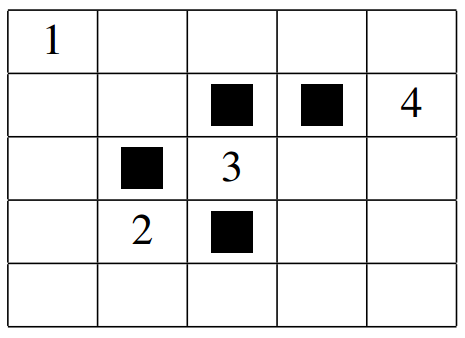
\includegraphics[width=3.0cm]{joisc2014.png}
		\end{center}
	\end{block}
	\begin{block}{constraint}
		$H, W \le 2000, P, Q \le 2 \times 10^5.$
	\end{block}
\end{frame}
\begin{frame}{[JOISC2014] 水壶}
	\begin{block}{solution}
		根据“货车运输”,我们只要对$P$栋建筑求一棵最小生成树就能回答询问了。\\
		
		问题在于怎么建立两两建筑之间的连边。做一个BFS,对每个非障碍的格子求出:离这个格子最近的建筑是哪个以及这个最近距离,当相邻的两个格子的最近建筑不同时,便可以在这两栋建筑之间建立连边。(可以感性地理解为每栋建筑向外扩张势力范围,一旦范围接壤就会产生连边。)\\
		
		可以证明从上述的所有边中就能够建立最小生成树,而这些边的数量是$O(HW)$的,规模在可接受范围内,可以使用Kruskal算法求出最小生成树,其中排序可以采用基数排序。		
	\end{block}
\end{frame}

\begin{frame}{[NOI2018] 归程}
	\begin{block}{description}
		一张$n$点$m$条边的无向图,每条边有具有长度和海拔。
		
		有$q$次询问,每次询问给出起始位置$v$和海拔下限$p$,你在$v$处有一辆车,车只能经过所有海拔不低于$p$的边,你可以选择把车停在任意位置,然后下车步行(没有海拔限制)回到$1$号点。
		
		要求对于每次询问,最小化步行距离。\textbf{强制在线}。
	\end{block}
	\begin{block}{constraint}
		$n \le 2 \times 10^5, m, q \le 4 \times 10^5.$
	\end{block}
\end{frame}
\begin{frame}{[NOI2018] 归程}
	\begin{block}{solution}
		相当于是求“从$v$出发经过海拔大于等于$p$的边能到达的所有点中,与$1$号点距离的最小值”。先通过一遍最短路求出每个点到$1$号点的距离$dis_i$。\\
		
		介绍一下Kruskal重构树,其主要思想就是对Kruskal算法中并查集的连边过程显式地建立出树结构,这样上述“从$v$出发经过海拔大于等于$p$的边能到达的所有点中”就对应并查集连边过程中某个时刻出现的一个连通块,这在Kruskal重构树上恰好对应一棵子树。\\
		
		因此只需要通过二分来定位子树,并维护子树内$dis_i$的最小值即可。
	\end{block}
\end{frame}

\begin{frame}{例题:位运算最优生成树}
	\begin{block}{description}
		给出$n$个数$\{a_i\}_{i=1}^{n}$,建立一张完全图,边$(i, j)$的边权是$a_i \oplus a_j$,其中$\oplus$是任意一个满足交换律的位运算(通过每一位上的真值表来给出)。
		
		求这张图的$\mathrm{optimal = \{maximal, minimal\}}$生成树。
	\end{block}
	\begin{block}{constraint}
		$n \le 10^5, 0 \le a_i < 2^{18}.$
	\end{block}
	\begin{block}{derivatives}
		$\oplus = \mathrm{bitwise\ xor}, \mathrm{optimal = minimal} \Rightarrow $ \href{http://codeforces.com/problemset/problem/888/G}{CodeForces888G Xor-MST}
		
		$\oplus = \mathrm{bitwise\ and}, \mathrm{optimal = maximal} \Rightarrow $ \href{https://uoj.ac/problem/176}{UOJ176 新年的繁荣}
	\end{block}
\end{frame}
\begin{frame}{例题:位运算最优生成树}
	\begin{block}{solution}
		(部分衍生问题存在复杂度更优的解法。)\\
		
		考虑一种统一的做法,考虑使用Borüvka算法。我们每轮需要做的事情是对每个$a_i$,找到一个异色的(不在同一个连通块内)$j$来最大/小化$a_i \oplus a_j$。\\
		
		位运算可以贪心,按照二进制位从高到低,我们每次希望当前的最高位能(填$1$/填$0$/填什么都行)。建立一棵Trie树,这样“填$1$/填$0$”只需要向特定的一边递归即可,而“填什么都行”就比较麻烦,需要预先处理一个Trie树合并,从而让往一边递归实际上起到了往两边递归的效果。\\
		
		需要注意的是Trie树每个节点上需要维护其子树内的两种不同颜色(因为要找且仅要找异色)。该算法的时间复杂度为$O(n\log n\log a_i)$。
	\end{block}
\end{frame}

\begin{frame}{「LibreOJ NOI Round \#2」签到游戏}
	\begin{block}{description}
		有一列数$\{A_i\}_{i=1}^{n}$,这些数你不知道,你需要猜它们的值。

		又有一列数$\{B_i\}_{i=1}^{n}$,这些数你知道。你可以选择支付$\gcd_{i=l}^{r}B_i$的代价,得到$\sum_{i=l}^{r}A_i$的值。

		\begin{itemize}
			\item 求至少需要支付多少代价,能保证准确猜出每个$A_i$?
			\item 有$q$次动态的询问,每次询问会修改$\{B_i\}$的一位,并求上一问的答案。
		\end{itemize}
	\end{block}
	\begin{block}{constraint}
		$n, q \le 10^5, 1 \le B_i \le 10^9.$
	\end{block}
\end{frame}
\begin{frame}{「LibreOJ NOI Round \#2」签到游戏}
	\begin{block}{solution}
		问题等价于有一张$n + 1$个点的图$G$,其中点$i, j(0 \le i < j \le n)$之间的边权是$\gcd_{k=i+1}^{j} B_k$,求$G$的最小生成树边权和。\pause\\
		
		验证:$G$存在一棵最小生成树$T$,包含边$(0, n)$,且对于任意$i = 1, 2, \cdots, n-1$,要么包含边$(0, i)$,要么包含边$(i, n)$。进一步地,存在分界点$1 \le x \le n$,$\forall y < x, (y, n) \in T, \forall y \ge x, (0, y) \in T.$\pause\\

		二分分界点$x$即可。使用线段树维护$\{B_i\}$,在线段树上二分即可求出分界点。之后需要实现求$\sum_{i=x}^{n}\gcd_{j=1}^{i}B_j$,注意到随着$i$的增加$\gcd_{j=1}^{i}B_j$只会变化至多$\log B_1$次,在线段树上找到这$\log B_1$次变化的位置即可。

	\end{block}
\end{frame}


\section{最短路}
\begin{frame}{最短路}
	BFS:解决所有边权都相同的问题,复杂度$O(m)$。\\
	
	Floyed:复杂度$O(n^3)$,需要注意的是三层循环的枚举顺序,以及当最外层循环变量\texttt{k}枚举到$k$时,数组中\texttt{dis[i][j]}表示的含义是:从$i$到$j$经过编号不超过$k$的中间节点的最短路。\\
	
	Dijkstra:解决边权非负的问题,可以通过堆优化得到$O(m\log m)$的复杂度。\\
	
	Bellman-Ford:进行$n$轮松弛操作(因为最短路的边数不会超过$n$),复杂度$O(nm)$,可以使用队列优化,但理论复杂度无法变优。
	\begin{itemize}
		\item 当使用(队列优化的)Bellman-Ford算法判负环时,正确的做法是记录最短路经过的边数,当边数大于$n$时便说明找到了负环。
	\end{itemize}
\end{frame}
\begin{frame}{最短路}
	
	01最短路(所有边边权$\in \{0,1\}$)可以做到$O(m)$。
	\begin{itemize}
		\item 类似 BFS 的过程,遇到$1$边就丢到队列末尾,遇到$0$边就丢到队列开头。
	\end{itemize}

	进一步的,所有边边权$\in [0,k]$的最短路问题可以做到$O(km)$。
	\begin{itemize}
		\item 和前者类似,维护$k+1$个队列即可。
	\end{itemize}

	更进一步的,$m_1$条边边权$\in [0, k]$,$m_2$条边边权不受限的最短路问题可以做到$O(km_1 + m_2\log m_2)$。	
	
\end{frame}

\begin{frame}{最短路树}
	这其实是非常简单的东西,就是根据最短路的更新关系建出来的一个树形结构。\\
	
	只是希望大家对这玩意儿能有个印象。
\end{frame}

\begin{frame}{[CERC2012] Farm and Factory}
	\begin{block}{description}
		有一张$n$点$m$条边的无向图,你需要新增一个点并向其余的部分点连边(边权可以是任意实数),使得任何其他的点到$1, 2$两个点的最短路都\textbf{可以不经过}这个新点,要求最小化新点到其余每个点的距离之和。
	\end{block}
	\begin{block}{constraint}
		$n \le 10^5, m \le 3 \times 10^5.$
	\end{block}
\end{frame}
\begin{frame}{[CERC2012] Farm and Factory}
	\begin{block}{solution}
		“任何其他的点到$1, 2$两个点的最短路都\textbf{可以不经过}新点”这个奇怪的限制实际上是限制了新点的加入不会改变原图中$1, 2$两点的最短路。\\
		
		设每个点$i$(自然不包括新点)到$1$的最短路是$f_i$,到$2$的最短路是$g_i$,到新点的最短路是$s_i$,我们可以得到对于每个$i$,都有$pair(f_i, s_i, s_1), pair(g_i, s_i, s_2)$这两个三元对满足三角不等式(即任两者之和不小于第三者)。\\
		
		因为要最小化$\sum s_i$,所以我们令$s_i = \max\{|f_i - s_1|, |g_i - s_2|\}()$一定不会劣。\\
		
		所以我们只需要确定$s_1, s_2$的取值,然后最小化$\sum \max\{|f_i - s_1|, |g_i - s_2|\}$就可以了。这个形式恰好是点$(s_1, s_2)$与点$(f_i, g_i)$的Chebyshev距离,只需要先转成Manhattan距离(这样两维就独立了),然后对两维坐标分别取中位数即可。
	\end{block}
\end{frame}

\begin{frame}{CodeChef Querying on a Grid}
	\begin{block}{description}
		一张$M \times N$的格点(不是格子)图,每条边有个非负边权,根据这个边权可以定义两个格点之间的最短路。
		
		有$Q$次如下两种操作:一种操作是给出两个格点,把两点间最短路上的所有格点的点权加上一个数(点权与最短路无关,这种操作保证\textbf{给出的两格点间最短路唯一}),另一种是查询某个格点的权值。
	\end{block}
	\begin{block}{constraint}
		$M \le 3, N, Q \le 10^5.$
	\end{block}
\end{frame}
\begin{frame}{CodeChef Querying on a Grid}
	\begin{block}{solution}
		一个显然的性质是对于任何$j \in [y_1, y_2]$,都存在某个$i \in [1, M]$,使得从$(x_1, y_1)$到$(x_2, y_2)$的最短路经过$(i, j)$。\\
		
		考虑分治,以$(i, mid), i \in [1, M]$作为起点求出到整张图的最短路,便可以得到所有跨越$mid$的点对间的最短路,然后左右两侧分别递归。\\
		
		上面求出了最短路的长度,怎么确定出这条路径呢?只需要建立出最短路树,那么这条路径就对应了最短路树上一条经过根(起点)的路径。\\
		
		需要支持的操作是树上的链加法和单点查询,可以差分为单点加法和子树查询,从而可使用树状数组维护。\\
		
		注意修改的时候只在一棵最短路树上做加法操作,而查询时需要在多棵最短路树上查询一个点的权值和。总时间复杂度为$O(M(N+Q)\log^2 N)$。
	\end{block}
\end{frame}

\begin{frame}{BZOJ4289 Tax}
	\begin{block}{description}
		一个 $n$ 个点 $m$ 条边的无向图,每经过一个点,产生的代价是进入和离开这个点的两条边的边权的较大值。
		
		求从起点 $1$ 到点 $n$ 的最小代价和。起点的代价是离开起点的边的边权,终点的代价是进入终点的边的边权。
	\end{block}
	\begin{block}{constraint}
		$n \le 10^5, m \le 2 \times 10^5.$
	\end{block}
\end{frame}
\begin{frame}{BZOJ4289 Tax}
	\begin{block}{solution}
		把题目中的边看成点,暴力建图会使边数达到平方级别。\\
		
		将$\max(a,b)$写成$a+\max(b-a,0)$,先直接计算进入时的边的代价,接着如果$b>a$就再加上一些代价。\\
		
		可以采用板书中的方式建图。
	\end{block}
\end{frame}
\begin{frame}{[SDOI2017] 天才黑客}
	\begin{block}{description}
		有一张$n$点$m$条边的有向图,每条边都有一个边权以及一个字符串,字符串的给出形式是给出一棵$k$个节点的Trie树上的某个节点。
		
		定义一条路径的权值是每条边的权值之和,加上任意相邻两条边上字符串的最长公共前缀(Longest Common Prefix, LCP)长度之和。
		
		求$1$号点到其余每个点的最小路径权值。
	\end{block}
	\begin{block}{constraint}
		$n, m, k \le 10^5.$
	\end{block}
\end{frame}
\begin{frame}{[SDOI2017] 天才黑客}
	\begin{block}{solution}
		两个字符串的LCP长度对应到Trie树上就是两点的LCA深度,也是两点欧拉序区间中深度的\obj{最小值}。\\
		
		在原图中的每个点上,对其入边与出边用到的点集建立Trie树的一棵虚树,按欧拉序排序后得到点列$p_1, p_2, \cdots, p_s$。我们希望建立一个结构,使得这个结构从$p_x$点进入、$p_y$点离开的最短路长度是$\min_{i=\min\{x, y\}}^{\max\{x, y\}}dep_{s_i}$。
		
		\begin{center}
			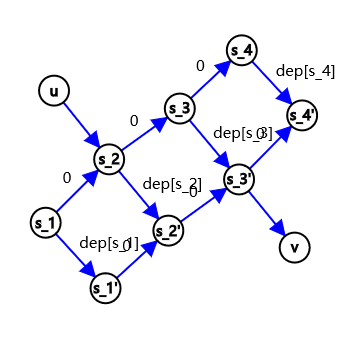
\includegraphics[width=3.0cm]{hacker.png}
			{\tiny \color{gray} 图有点丑,用CSAcademy上的graph\_editor随手画的}
		\end{center}
		
		上图解决了$x \le y$的情况,可以对称地解决另外一半。
		
	\end{block}
\end{frame}


\begin{frame}{Luogu2371 墨墨的等式}
	\begin{block}{description}
		对于方程$\sum_{i=1}^na_ix_i = b$,求有多少满足$b \in [l,r]$的$b$使方程存在非负整数解。
	\end{block}
	\begin{block}{constraint}
		$n \le 12, 0 \le a_i \le 5 \times 10^5, 1 \le l \le r \le 10^{12}.$
	\end{block}
\end{frame}
\begin{frame}{Luogu2371 墨墨的等式}
	\begin{block}{solution}
		选$a_1$作为基,显然若$b$满足条件,则$b+a_1$也满足。\\
		
		记$f_i$表示用$a_2,a_3,...,a_n$能凑出的最小的模$a_1$等于$i$的数,这部分可以使用最短路算法解决。求出了$f_i$后也便不难求出$[l,r]$中合法$b$的数量。\\
		
		这个东西往往被称为同余类最短路问题,17年人尽皆知的$a\times b - a - b$本质上也属于这类问题。
	\end{block}
\end{frame}

\section{Tarjan}
\begin{frame}{Tarjan全家桶}
	一般来说包含求(无向图)点双连通分量、边双连通分量以及(有向图)强连通分量。\\
	
	算法流程大致可以概括为:建立一棵 DFS 树,对每个节点记录访问时间$dfn_i$以及其 DFS 树子树内节点通过\textbf{一条返祖边}能够到达节点的最小$dfn$。注意在无向图中只存在树边和返祖边,有向图中存在树边、返祖边以及横跨边。\\
	
	算法竞赛领域对Tarjan相关算法的考察点一般为:
	
	\begin{itemize}
		\item 点双连通分量 $\to$ 圆方树 $\to$ 相关树上算法
		\item 边双连通分量 $\to$ 树 $\to$ 相关树上算法
		\item 强连通分量 $\to$ DAG $\to$ DAG上动态规划
	\end{itemize}
	
	一个点唯一存在于一个边双或者强连通分量,但可能存在于多个点双连通分量。
	
\end{frame}

\begin{frame}{圆方树}
	圆方树是一种能够表示点双连通关系的树结构。
	
	\begin{center}
		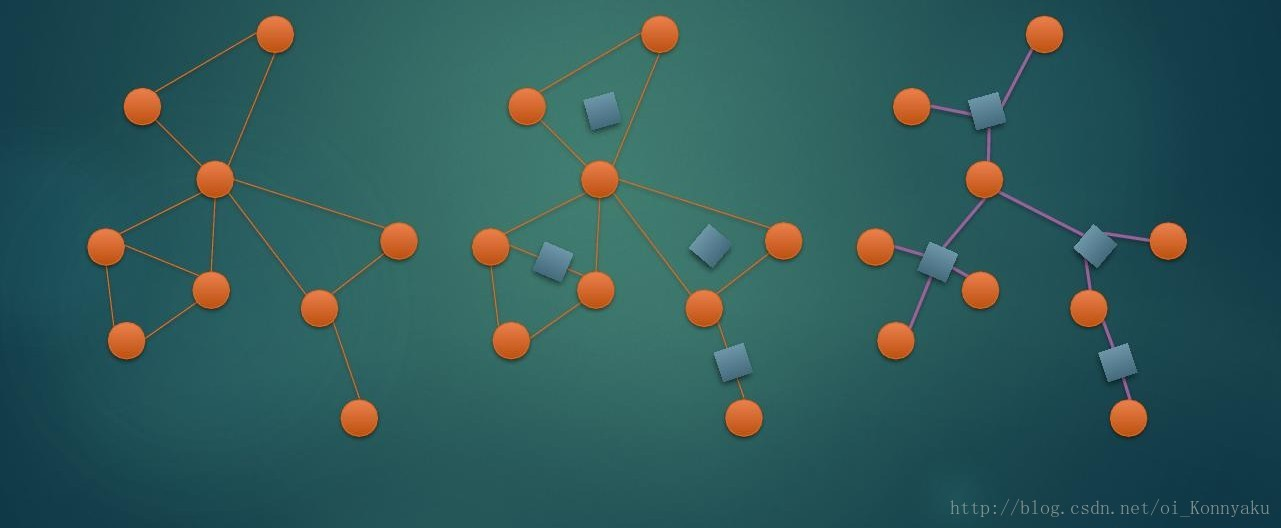
\includegraphics[width=9.0cm]{yuanfangshu.jpg}
	\end{center}

	构建方式为:把原图的中的点看作圆点,对图中的每个点双新建一个方点并向其内部所有圆点连边,随后删除点双中原有的边,只保留一个菊花的结构。\\
	
	如此以来任意两点间路径上的圆点便是割点,或者说必经点。
\end{frame}

\begin{frame}{[JSOI2012] 越狱老虎桥}
	\begin{block}{description}
		一张$n$点$m$条边的无向图,边有边权。
		
		Alice会往图中加入一条边,然后Bob会选择割掉图中的一条边使得图不连通(不能割Alice加的那条边)。
		
		Bob希望最小化割掉的边权,Alice希望最大化,求最终被割掉的边权。
	\end{block}
	\begin{block}{constraint}
		$n, m \le 10^6.$
	\end{block}
\end{frame}
\begin{frame}{[JSOI2012] 越狱老虎桥}
	\begin{block}{solution}
		首先边双里的边都不能割,那么把边双缩点,问题被放到了树上。\\
		
		Alice如果选择了加入边$(u, v)$,那么Bob就不能割树上$u, v$路径上的所有边(因为割了之后图还是连通的)。\\
		
		因此按边权从小到大标记树边,直到已标记的树边无法被一条链覆盖为止。无法被覆盖的最后一条边就是答案。
	\end{block}
\end{frame}

\begin{frame}{LOJ2480 One-Way Streets}
	\begin{block}{description}
		有一张$n$点$m$条边的无向连通图,你需要对每一条边定向。有$p$条限制,每条限制形如$x\to y$要求定向后存在从点$x$到点$y$的路径。你需要判断每条边是否可以被唯一定向,若可以,需给出唯一确定的方向。
	\end{block}
	\begin{block}{constraint}
		$n, m, p \le 10^5.$
	\end{block}
\end{frame}
\begin{frame}{LOJ2480 One-Way Streets}
	\begin{block}{solution}
		求边双,一个边双连通分量内的所有边的方向都是可任选的。\\
		
		边双缩点变成一棵树,那么问题就变成了树上从一点$x$要走到另一点$y$。树上差分即可。
	\end{block}
\end{frame}

\begin{frame}{UOJ30 Tourists}
	\begin{block}{description}
		一张$n$点$m$边无向图,每个点有一个点权,$q$次操作,每次操作为修改一个点的点权或者是询问两点$(u,v)$之间\textbf{所有简单路径}中经过的最小点权。
	\end{block}
	\begin{block}{constraint}
		$n, m, q \le 10^5.$
	\end{block}
\end{frame}
\begin{frame}{UOJ30 Tourists}
	\begin{block}{solution}
		建出圆方树,在每个方点上维护整个点双的最小点权,那么每次询问就是查询树上路径最小值。\\
		
		但是在有修改的时候,修改一个圆点的点权会导致它所有相邻方点受到影响,从而使复杂度退化。\\
		
		可以采取的解决方法是:方点中维护的信息不包含其父亲圆点,这样修改一个圆点只需要进一步修改其父亲方点,查询时也只需要在路径 LCA 是方点时额外计算一下其父亲圆点即可。
	\end{block}
\end{frame}
\subsection{2SAT}
\begin{frame}{\textrm{SAT}}
	由变量$u_1, \cdots, u_n$和逻辑运算 \textrm{AND}($\wedge$),\textrm{OR}($\vee$),\textrm{NOT}($\lnot$)组成的式子称为\obj{布尔表达式}。有一类特殊的布尔表达式,形如$\bigwedge_i \left(\bigvee_j v_{i_j}\right)$,其中$v_{i_j}$是某个变量$u_k$或者其否定$\lnot u_k$,称这种布尔表达式为\obj{合取范式(Conjunctive Normal Form, CNF)}。\\

	当确定了每个变量的$\{0, 1\}$取值后,布尔表达式存在真值 \textrm{TRUE} 或者 \textrm{FALSE}。称一个布尔表达式是\obj{可满足的},如果存在一个变量取值使得布尔表达式的真值为 \textrm{TRUE}。\\

	{SAT} 问题就是判断给定的 \textrm{CNF} 是否可满足。特别的,定义 $k$\textrm{CNF} 为每个子句中包含不超过$k$个变量或其否定的 \textrm{CNF},$k$\textrm{SAT} 问题就是判断给定的 $k$\textrm{CNF} 是否可满足。
\end{frame}
\begin{frame}{$2$\textrm{SAT}}
	在 Complexity Theory 中,Cook-Levin Theorem 指出 \textrm{SAT} 和 $3\mathrm{SAT}$ 是 \textbf{NP} 完全的。所以我们只考虑研究 $2$\textrm{SAT} 的解法。\\

	考虑 $2$\textrm{SAT} 中的一个子句,必然形如 $u_i \vee u_j$ 或者 $u_k$。前者等价于$\lnot u_i \Rightarrow u_j$以及$\lnot u_j \Rightarrow u_i$,后者等价于$\lnot u_k \Rightarrow u_k$\footnote{\tiny 蕴含($\Rightarrow$) 并不是基础的逻辑运算,但可以由后者定义,同时也更加符合直觉。}。\\

	$a \Rightarrow b$ 的含义是如果 $a$ 为 \textrm{TRUE} 则 $b$ 也为 \textrm{TRUE}。把 $a \Rightarrow b$ 理解成图论模型中一条从 $a$ 到 $b$ 的边,那么一个 $n$ 元变量的 $2$\textrm{CNF} $\varphi$ 可以对应建立出一张 $2n$ 个点的有向图 $G_{\varphi}$。\\
	
	一个使 $\varphi$ 为 \textrm{TRUE} 的变量取值对应\footnote{\tiny 这个对应还是比较自然的,只需要把$S$中的变量设成$1(\mathrm{TRUE})$就行了。} $G_{\varphi}$ 的一个子集$S$,满足
	\begin{itemize}
		\item $\forall i \in [1, n]$,$u_i \in S$和$\lnot u_i \in S$恰有一者成立。
		\item $S$是闭合的,即$\forall a, b \in G_{\varphi}$,如果$a \in S$且$a$可达$b$,则$b \in S$。
	\end{itemize}
\end{frame}
\begin{frame}{$2$\textrm{SAT}}
	\begin{theorem}
		$n$ 元变量的 $2$\textrm{CNF} $\varphi$ 可满足,当且仅当$\forall i \in [1, n]$,$u_i$ 和 $\lnot u_i$ 在 $G_{\varphi}$ 中\obj{不强连通}。
	\end{theorem}\pause
	\begin{proof}
		必要性显然。直接考虑构造证明充分性:

		对 $G_{\varphi}$ 缩点得到一个 DAG $G_{\varphi}'$,我们指出$G_{\varphi}'$的所有强连通分量存在某种“对称性”:如果某个强连通分量$C$包含变量$u_{i_1}, \cdots, u_{i_k}$,则一定存在另外一个强连通分量$\lnot C$包含变量$\lnot u_{i_1}, \cdots, \lnot u_{i_k}$。
		
		对 $G_{\varphi}'$ 做拓扑排序,对每对 $(C, \lnot C)$选择拓扑序较大的一者加入$S$。此时 $S$ 满足前一页陈述的两个条件,从而说明 $\varphi$ 可满足。

		\begin{itemize}
			\item $u_i$ 和 $\lnot u_i$ 不属于同一个强连通分量,故 $S$ 恰包含其一者。
			\item 假设 $S$ 不闭合,则可以由 $G_{\varphi}$ 的对称性导出矛盾。
		\end{itemize}

		$G_{\varphi}$ 的对称性是指$(u_i, u_j) \in G_{\varphi} \Leftrightarrow (\lnot u_j, \lnot u_i) \in G_{\varphi}$。
	\end{proof}
\end{frame}
\begin{frame}{$2$\textrm{SAT}}
	前述的构造性证明已经给出了 $2$\textrm{SAT} 的具体解法。值得一提的是,在调用 Tarjan 算法缩点的过程中,强连通分量会被按某个\obj{拓扑序逆序}标记,从而“拓扑序较大”等价于“强连通分量标号较小”,说明并不需要显式地进行拓扑排序。
\end{frame}
\begin{frame}{UOJ210 寻找罪犯}
	\begin{block}{description}
		$n$ 位嫌疑人提供了总共 $m$ 条供词,每条供词都形如“$x_i$ 号嫌疑人说 $y_i$ 号嫌疑人是/不是罪犯”。已知罪犯会恰好说一句假话,而清白的人不会说假话。要求判断哪些人是罪犯,输出任意一组合法解。
	\end{block}
	\begin{block}{constraint}
		$n, m \le 10^5.$
	\end{block}
	\pause
	\begin{block}{solution}
		$crime_i$ 表示 $i$ 号嫌疑人是不是罪犯,$fake_{i,j}$ 表示 $i$ 号嫌疑人说的前 $j$ 句话里有没有假话。设第$i$个人说的第$j$句话是“$x_{i, j}$不是罪犯”\footnote{\tiny 如果说的是“不是罪犯”就用$\lnot crime_{x_{i,j}}$替换$crime_{x_{i,j}}$。}
		\begin{align*}
			\varphi = \bigwedge_{i,j} &(crime_{x_{i,j}} \Rightarrow crime_i) \wedge (crime_{x_{i,j}} \Rightarrow fake_{i,j}) \\ \wedge &(crime_{x_{i,j}} \Rightarrow \lnot fake_{i,j-1}) \wedge (fake_{i,j} \Rightarrow fake_{i, j+1})
		\end{align*}
	\end{block}
\end{frame}

\section{二分图}
\begin{frame}{二分图匹配}
	$G = \langle V_1, V_2, E\rangle$ 其中 $E \subseteq V_1 \times V_2$ 称为二分图。一张图是二分图当且仅当它不存在奇环。\pause\\
	
	二分图$G(V_1, V_2, E)$的一个匹配是一个一一对应$\sigma: S_1 \to S_2$,其中$S_1 \subseteq V_1, S_2 \subseteq V_2$,且$\forall v \in S_1, (v, \sigma(v)) \in E$。最大匹配$\sigma_{\max}$就是使$|\sigma|$取到最大的$\sigma$。\pause\\
	
	解决二分图最大匹配的常用算法是匈牙利算法,其思路是从$V_1$的一个未匹配点出发,\obj{“从左向右走未匹配边”},\obj{“从右向左走匹配边”},如果存在一条路径最终到达$V_2$的一个未匹配点,则该路径长度为奇数且匹配边与未匹配边交错(称之为\obj{交错路}),因此可将该路径上所有边的匹配状态取反,便使匹配数量增加$1$。\\
	
	由于单次运行复杂度最坏为$O(m)$,需运行$n$次,故匈牙利算法解决二分图匹配问题的复杂度为$O(nm)$。若使用 dinic 优化的网络流算法解决二分图匹配问题,时间复杂度为$O(m\sqrt n)$。
	
\end{frame}

\begin{frame}{可行点与必经点}
	\begin{block}{可能在最大匹配中的点}
		\pause
		所有有度数的点都可能在最大匹配中。
	\end{block}
	\pause
	\begin{block}{一定在最大匹配中的点}
		\pause
		先求出任意一组最大匹配$S$,那么一定在最大匹配中的点构成的集合就是$S$的子集。
		
		以左侧点为例,一个属于集合$S$的左侧点$x$可能不在最大匹配中当且仅当存在一个不属于集合$S$的左侧点$y$满足$y$到$x$存在一条交替路。右侧点同理。
		
		或者说,建立匹配$S$的残量网络,从源点能到达的$S$中左侧点以及能到达汇点的$S$中右侧点都可能不在最大匹配中。
		
		其他的点都一定在最大匹配中。
	\end{block}
\end{frame}

\begin{frame}{可行边与必经边}
	\begin{block}{可能在最大匹配中的边}
		\pause
		先求出任意一组最大匹配$S$,$S$中的边都可能在最大匹配中。
		
		其余的边需要考虑两种情况:一种是连接已匹配点和未匹配点的边,这种边一定可以换到匹配中;另一种连接两个已匹配点,要使它出现在匹配中需要找出一个\obj{交错环}。
		
		依然建立残量网络,上述第二种情况等价于连接的两点在同一个强连通分量中(其实第一种情况也满足)。
	\end{block}
	\pause
	\begin{block}{一定在最大匹配中的边}
		\pause
		依旧是求出任意一组最大匹配$S$,答案是$S$的子集。
		
		从源点能到达的匹配边和能到达汇点的匹配边都可能不在最大匹配中。这是匹配点变更造成的影响。
		
		还需要考虑交替环的影响。连接两端点在同一个强连通分量中的匹配边也可能不在最大匹配中。
	\end{block}
\end{frame}
\begin{frame}{[TJOI/HEOI2016] 游戏}
	\begin{block}{description}
		一张$n \times m$的网格图,每个格子都是空地、墙壁或是草丛中的一种。
		
		你可以选择在空地上安放炸弹,炸弹的爆炸范围是从安放炸弹的格子出发向上下左右四个方向延伸直至碰到墙壁或者离开网格图(注意草丛是可以被炸弹穿过的)。
		
		问最多可以安放多少炸弹,使得任意两个炸弹不会互相炸到。
	\end{block}
	\begin{block}{constraint}
		$n, m \le 50, \mbox{墙壁数量}\le 300.$
	\end{block}
\end{frame}
\begin{frame}{[TJOI/HEOI2016] 游戏}
	\begin{block}{solution}
		一行或一列连续的空地/草丛中只能放置至多一个炸弹。\\
		
		题意可以抽象成:选尽量多的空地(放置炸弹),满足这些空地两两不在同一个行或列的连续段中。\\
		
		把行连续段看成二分图一侧的点,列连续段看成二分图另一侧的点,空地看成连接两者的边,便转化成了二分图最大匹配问题。
	\end{block}
\end{frame}
\begin{frame}{二分图的最大独立集和最小覆盖集}

	$|$最小覆盖集$|$ $\ge$ $|$最大匹配$|$。如若不然,匹配边无法覆盖。

	通过构造证明上式取等:先求出一组最大匹配,从$V_1$中的所有未匹配点出发 DFS,从左往右走非匹配边,从右往左走匹配边。取$V_1$中的未访问点和$V_2$中的已访问点构成集合$S$。\pause

	\begin{itemize}
		\item $|S| = $ $|$最大匹配$|$。因为$S$中的点一定都在匹配中,且对于每条匹配边,都有恰好一个点在$S$中。
		\item $S$是覆盖集。即不存在一条边$(x \in V_1, y \in V_2)$,$x$已访问且$y$未访问。
		\begin{itemize}
			\item 这条边是匹配边。$x$是匹配点,所以不会从$x$出发 DFS,$x$被访问依赖于其匹配点$y$被访问,矛盾;
			\item 这条边是非匹配边。此时访问到$x$时也会沿这条边访问到$y$,矛盾。
		\end{itemize}
	\end{itemize}

	于是构造出了大小等于最大匹配的覆盖集。\pause

	可以验证任意独立集的补集都是覆盖集,所以最大独立集可以规约到最小覆盖集。

\end{frame}
\subsection{KM算法}
\begin{frame}{KM算法}
	$G = \langle V_1, V_2, w: V_1 \times V_2 \to \mathbb R \rangle$称为带权二分图。不妨假设$|V_1| = |V_2|$,如何求匹配$\sigma: V_1 \to V_2$来最大化$\sum_{v \in V_1}w(v, \sigma(v))$?\\

	类似匈牙利算法,仍然考虑为左侧的未匹配点找\obj{交错路}\footnote{\tiny 但可不是乱找啊,显然我们得有备而来。}\pause\\

	称满足$\forall (u, v) \in V_1 \times V_2, \mathrm{label}(u) + \mathrm{label}(v) \ge w(u, v)$的函数$\mathrm{label}: V_1 \cup V_2 \to \mathbb R$为合法的顶标函数。由$G$和一个合法的顶标函数$\mathrm{label}$可以导出一张二分图$G' = \langle V_1, V_2, E \rangle$其中$(u, v) \in E \Leftrightarrow \mathrm{label}(u) + \mathrm{label}(v) = w(u, v)$。

	\begin{lemma}
		若上述$G'$存在$|\sigma| = |V_1|$的匹配$\sigma$,则$\sigma$也是$G$的最大权匹配。
	\end{lemma}
\end{frame}
\begin{frame}{KM算法}
	根据引理,我们只需要找到一个合法的$\mathrm{label}$满足$G'$有完美匹配就行了。构造方式是调整,从一个平凡的合法$\mathrm{label}$出发:$$\mathrm{label}_0(v) = \begin{cases}
		\max_{v' \in V_2}w(v, v'), & v \in V_1\\
		0, & v \in V_2
	\end{cases}$$

	维护$G'$的一个匹配$\sigma$,每次从$V_1$的一个未匹配点$v$出发找交错路。交错路可能找不到,其关键在于$\mathrm{label}$限制了更多的$V_2$的点被探索到。假设从$v$出发能探索到的点集为$S$,则修改$\mathrm{label}$为$\mathrm{label}'$:
	$$\mathrm{label}'(v) = \begin{cases}
		\mathrm{label}(v) - a, & v \in S \cap V_1\\
		\mathrm{label}(v) + a, & v \in S \cap V_2\\
		\mathrm{label}(v), & \textrm{otherwise}\\
	\end{cases}$$
	其中$a > 0$。
\end{frame}
\begin{frame}{KM算法}
	陈述如下事实:
	\begin{itemize}
		\item $G' \Leftarrow (G, \mathrm{label})$的匹配$\sigma$仍是$G'' \Leftarrow (G, \mathrm{label}')$的匹配。
		\item 若取$a = \min\limits_{v \in V_2 \setminus S} \min\limits_{u \in S \cap V_1} \textrm{label}(u) + \mathrm{label}(v) - w(u, v)$,则$\mathrm{label}'$仍是合法顶标,且修改后$S$能够扩大。
	\end{itemize}

	上述$a$的取值就是“从左边探索右边一个新点所需要的最小代价”,一般会考虑维护$\mathrm{slack}(v) = \min\limits_{u \in S \cap V_1} \textrm{label}(u) + \mathrm{label}(v) - w(u, v)$。\\

	用 BFS 实现上述过程。由于对每个$v \in V_1$,找交错路的复杂度都不超过把整张图遍历一边,所以该算法的时间复杂度为 $O(n^3)$,与匈牙利算法是一致的。

\end{frame}


\subsection{Hall 定理}
\begin{frame}{Hall 定理}
	\begin{theorem}
		二分图$G = \langle V_1, V_2 \rangle $存在\obj{饱和}$V_1$的完美匹配,当且仅当对于$\forall S \subseteq V_1, |\mathcal N(S)| \ge |S|$,其中$\mathcal N(S) = \bigcup_{v \in S}\mathrm{adj}(v)$。
	\end{theorem}
	\begin{proof}
		必要性显然。充分性考虑对$|V_1|$归纳。
		\begin{itemize}
			\item 如果存在$S \subsetneq V_1$满足$|\mathcal N(S)| = |S|$,根据归纳假设$G' = (S, \mathcal N(S))$存在完美匹配,且可验证$G'' = (V_1 \setminus S, V_2 \setminus \mathcal N(S))$符合定理条件,故也存在完美匹配,从而也存在完美匹配,故$G = (V_1, V_2)$存在完美匹配。
			\item 如果$\forall S \subsetneq V_1$都有$|\mathcal N(S)| > |S|$,那么随便匹配一条边仍满足定理条件,根据归纳假设存在完美匹配。
		\end{itemize}
	\end{proof}

	OI 中常见的使用方式是将任意子集的限制“弱化”成任意区间,并证明“并不会真的弱化”。
	
\end{frame}

\begin{frame}{300iq Contest 1 Dates}
	\begin{block}{description}
		这道题需要一个主人公,我们不妨管他叫小X。
		
		在接下来的$m$天时间里,有$n$个人想要和小X约会。第$i$个人想要在$[l_i,r_i]$中的某一天和小X约会,且约会后小X会得到$p_i$的愉悦值。
		
		\textbf{在这里,我们保证$l_i\le l_{i+1}, r_i \le r_{i+1}$}。
		
		小X在第$i$天至多和$a_i$个人约会,他希望你帮他求出他能获得的最大愉悦值之和。
	\end{block}
	\begin{block}{constraint}
		$n, m \le 3\times 10^5, 0 \le a_i \le n, 1 \le p_i \le 10^9.$
	\end{block}
\end{frame}
\begin{frame}{300iq Contest 1 Dates}
	\begin{block}{solution}
		按照$p_i$从大到小依次判断加入这个区间后是否仍存在完美匹配,这种做法的正确性显然。\\
		
		根据Hall定理,判断是否存在完美匹配,需要对$n$个区间的每个子集$S$,检验是否满足$\sum_{i \in S}b_i \le \sum_{\exists i \in S, j \in [l_i, r_i]}a_j$,其中$b_i \in \{0, 1\}$表示第$i$个区间有没有被选。注意到$\{l_i\}, \{r_i\}$的单调性,枚举$S$时只需要枚举$[1, n]$的子区间即可,即枚举$[L, R] \in [1, n]$,限制要求为$\sum_{i=L}^{R}b_i \le \sum_{j=l_L}^{r_R}a_j$。\\
		
		记$sa_i,sb_i$分别为$a_i$和$b_i$的前缀和,于是得到$sb_R-sb_{L-1}\le sa_{r_R}-sa_{l_L-1}$即$sb_R-sa_{r_R}\le sb_{L-1}-sa_{l_L-1}$。再记$c_i=sb_i-sa_{r_i},d_i=sb_{i-1}-sa_{l_i-1}$,限制为$c_R\le d_L$。\\
		
		考虑每次加入一个区间是企图将某一个$b_x$由$0$改为$1$,观察发现只会有$c_{x \cdots n}$与$d_{1 \cdots x}$的大小关系会受到影响,因而维护$\{c_i\}$的后缀最大值和$\{d_i\}$的前缀最小值判断即可。
	\end{block}
\end{frame}

\section{三元环计数}
\begin{frame}{无向图三元环计数}
	对一张无向图数有多少无序三元组$(x,y,z)$满足图中存在边$(x,y),(x,z)$以及$(y,z)$。\pause\\
	
	对所有点按度数为第一关键字、标号为第二关键字排序,把所有边按照排序得到的排名重定向(排在前面的指向排在后面的),这样可以保证新生成的有向图是一个DAG,且每个点的出度不超过$\sqrt m$。\\
	
	枚举边$(A,B)$,先遍历$A$的所有出边并标记,再遍历$B$的所有出边,发现一个标记就说明找到了一个三元环。\\
	
	总时间复杂度是$O(m\sqrt m)$,同时也证明了$m$条边的无向图中的三元环数量是$O(m\sqrt m)$。
\end{frame}

\begin{frame}{HDU6144 Counting Stars}
	\begin{block}{description}
		一张$n$点$m$边无向图,求图中有多少个“A-structure”。
		
		一个“A-structure”被定义为一个有序的节点四元组$(A, B, C, D)$满足边$(A, B), (B, C), (C, D), (A, D), (A, C)$都存在于图中。
	\end{block}
	\begin{block}{constraint}
		$n, m \le 2 \times 10^5.$
	\end{block}
\end{frame}
\begin{frame}{HDU6144 Counting Stars}
	\begin{block}{solution}
		一个“A-structure”就是一对有一条边重合的三元环。\\
		
		用前面讲到过的办法数出每条边所处的三元环个数$cnt_i$,$\sum \binom{cnt_i}{2}$就是答案。
	\end{block}
\end{frame}
\begin{frame}{[POI2013] Price List}
	\begin{block}{description}
		有一张$n$点$m$条边的无向图,每条边的边权都是$a$。
		
		现在对这张图进行一些操作:对于所有在原图中最短距离为$2a$的点对$(i, j)$,加入一条连接$i, j$且边权为$b$的边。
		
		求这张新图中指定源点$S$到其余每个点的最短路。
	\end{block}
	\begin{block}{constraint}
		$n, m \le 10^5.$
	\end{block}
\end{frame}
\begin{frame}{[POI2013] Price List}
	\begin{block}{solution}
		可以发现新图上从$S$走到$T$的最短路的策略有且仅有如下三种:
		\begin{itemize}
			\item 只走$a$边,忽视加入的$b$边;
			\item 把两条$a$边并作一条$b$边走,最后视奇偶性可能会多出来一条$a$边;
			\item 只走$b$边。
		\end{itemize}
		
		前两种只需要对原图做一遍BFS。考虑第三种:当$u$点向外转移时,需要先枚举一个$u$的相邻点$v$,再枚举一个$v$的相邻点$w$,若$u, w$之间没有边,便可以从$u$来更新$w$。\pause
		
		注意这个过程中每个点只会被更新一次,所以一旦$u$成功更新$w$(等价于$u, w$之间没有边),$v \to w$这条枚举就可以删了。也即对于成功更新的部分,复杂度是关于一阶段枚举量线性的,也即$O(m)$。\pause
		
		问题在于不能成功更新的部分,即$u, w$之间有边,这说明$(u, v, w)$构成一个三元环,而三元环个数是$O(m\sqrt m)$的,每个三元环对枚举复杂度的代价又是常数,因此总时间复杂度为$O(m\sqrt m)$。
	\end{block}
\end{frame}



\section{欧拉回路}
\begin{frame}{欧拉回路}
	俗称一笔画。以下为了方便起见只讨论连通图上的问题。\\
	
	分无向图/有向图两种版本:无向图存在欧拉回路要求所有点的度数均为偶数;有向图则要求所有点入度等于出度。\\
	
	欧拉路不要求回到起点,要求除起点终点外其他点都是偶度点。可以理解为新加一条边连接起点终点后的欧拉回路。\pause\\
	
	多笔画(多条欧拉路)问题?\pause 奇度点两两匹配后求出欧拉回路,把新加的边删除后即得到了多条欧拉路。\pause\\
	
	建议先去 \href{https://uoj.ac/problem/117}{UOJ117} 写一份模板,你很可能因此找出代码中藏匿的bug......
	
\end{frame}

\begin{frame}{CodeForces429E Points and Segments}
	\begin{block}{description}
		有$n$个闭区间,你需要对每个区间进行黑白染色,使得任意一个点被不同颜色的区间的覆盖次数之差不超过 $1$ 。
	\end{block}
	\begin{block}{constraint}
		$n \le 10^5$,数据保证有解。
	\end{block}
\end{frame}

\begin{frame}{CodeForces429E Points and Segments}
	\begin{block}{solution}
		你能猜到这道题目和欧拉回路有关吗?\\
		
		记黑色区间的权值为$1$,白色为$-1$,等价于要求任意一个点被覆盖的所有区间的总权值 $\in [-1,1]$。\\
		
		对于区间$[l,r]$,从$l$向$r+\varepsilon$连一条边,并对所有奇度点按横坐标顺序两两连边(相当于加入了一些新区间),在新生成的图上求出欧拉回路,把从左往右的边染成黑色,从右往左的边染成白色,此时所有点被覆盖区间的总权值均为$0$。\\
		
		注意到新加入的区间集是\textbf{无交}的,因此只要直接去掉这些区间,便可以满足原题中权值$\in[-1,1]$的要求。
		
	\end{block}
\end{frame}
\section{网络流}
\begin{frame}{网络流}
	参考《网络流专题选讲》。
\end{frame}
\section{习题课}
\begin{frame}
	\begin{center}
		{\huge 习题课}
	\end{center}
\end{frame}
\begin{frame}{Gym102900K. Traveling Merchant}
	\begin{block}{description}
		有一张$n$个点$m$条边的无向图。每个点标有黑或白的颜色,每当离开一个点时,这个点的颜色就会发生翻转。

		你需要从$1$号点出发,黑白相间地走过一个节点序列。这里的颜色检查发生在进入节点时,保证$1$号点初始时是黑色。

		问是否存在一个无限长的黑白相间的节点序列。
	\end{block}
	\begin{block}{constraint}
		$n, m \le 2 \times 10^5.$
	\end{block}
\end{frame}
\begin{frame}{Gym102992D. Degree of Spanning Tree}
	\begin{block}{description}
		有一张$n$个点$m$条边的无向图。求它的一棵没有度数大于$2$的点的生成树,或者指明无解。
	\end{block}
	\begin{block}{constraint}
		$2 \le n \le 10^5, n - 1 \le m \le 2 \times 10^5.$
	\end{block}
\end{frame}
\begin{frame}{Gym102992M. Harmony in Harmony}
	\begin{block}{description}
		有一片面积为$1$的土地$D$。定义$D$的一个\obj{$n$等分}是一个集合族$\{A_i\}_{i=1}^{n}$,满足$\bigcup_{i=1}^{n}A_i = D$,且$\forall i \neq j, A_i \cap A_j = \varnothing$,同时每个$A_i$的面积\footnote{\tiny 感性理解一下什么是“面积”即可,严谨定义与解题关系不大。}均为$\frac 1n$。

		求$$\min_{\{S_i\}, \{T_i\}} \max_{\sigma \in \mathcal S_n} \min_{i=1}^{n} \mathrm{Area}(S_i \cap T_{\sigma_i})$$

		{\tiny 用自然语言表述一下:先Alice给出两个$n$等分,然后Bob给出这两个集合族之间的一个一一对应,定义评价指标值是对应的集合交(表示两块土地交的面积)的最小值,Alice希望这个值尽量小,Bob希望尽量大,求最终值是多少。}
	\end{block}
	\begin{block}{constraint}
		$n \le 500.$
	\end{block}
\end{frame}
\section{讲完啦}
\begin{frame}
	\begin{center}
		{\huge 谢谢大家!\\~\\  \large 祝大家学业有成!}
	\end{center}
\end{frame}

\end{document}